\chapter{Конструкторский раздел}
\label{cha:design}

В данном разделе будет приведено описание схемы конвейера.

\section{Схема конвейера}

Этот конвейер представляет собой простой конвейер обработки изображений.
Идея была взята из конвейера обработки изображений машинного обучения (сверточной сети).
На рисунке показана схема конвейера.
В конвейере рабочие одной стадии делят входные и выходные каналы.


\begin{figure}[h!]
    \centering
    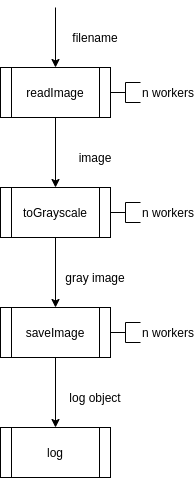
\includegraphics[width=0.3\textwidth]{5/inc/d1.png}
    \caption{Схема конвейера}
    \label{fig:2.2}
\end{figure}



\section{Вывод}
В данном разделе было приведено описание схем простого конвейера обработки изображений.
